\chapter{Prototype}
\section{Analysis}
The prototype has been chosen to be a service that distributes news tagged with one or more predefined categories,
e.g. sports, economy, and science; the subscribers may only be interested in certain news
categories, and for our prototype, the topics will be Tech and movies.

The prototype must at least involve:

\begin{enumerate}
  \item Two publishers that publishes different kinds of data.
  \item Two subscribers with different data needs.
  \item Differentiated levels of quality of service.
\end{enumerate}

\begin{figure}[ht!]
\centering
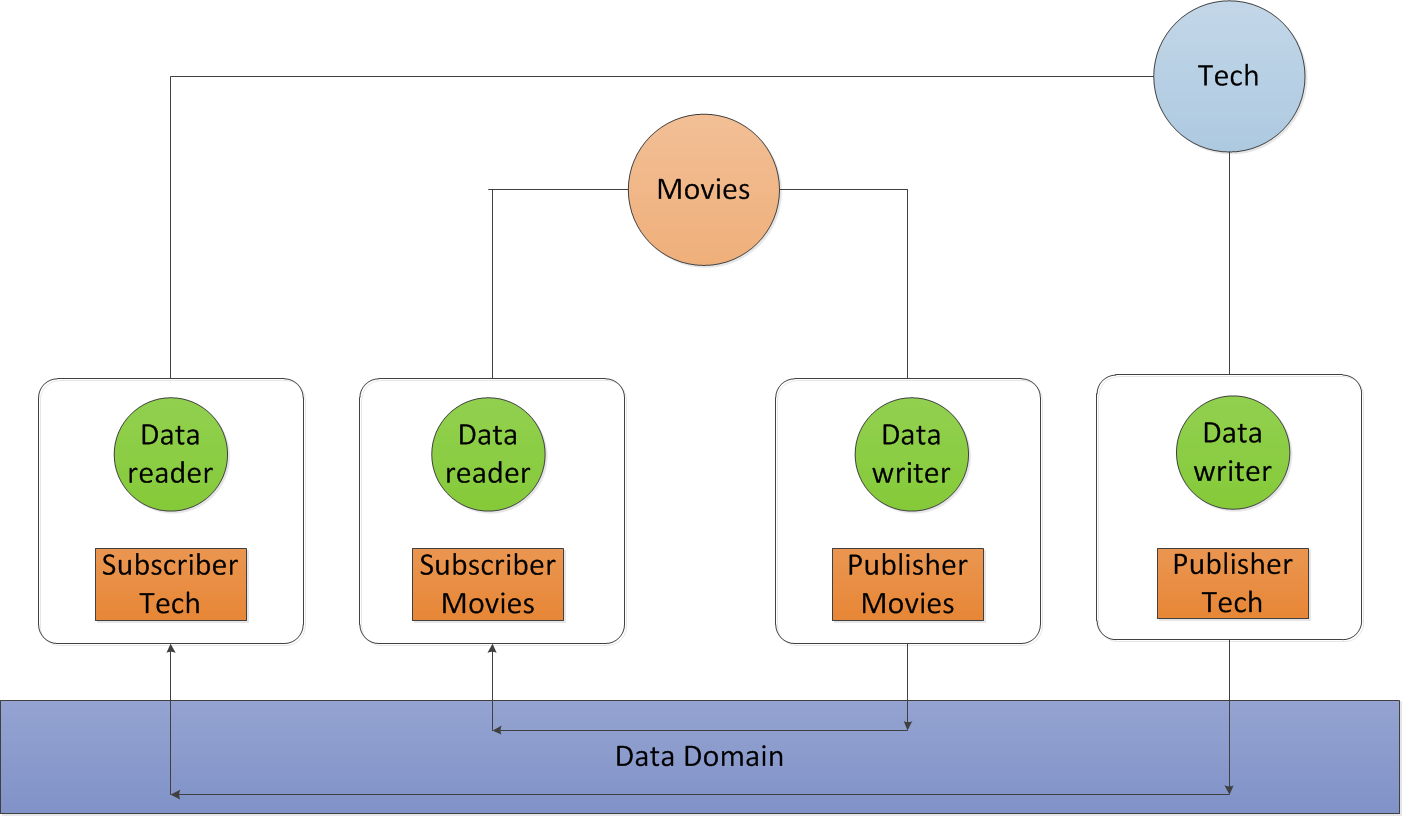
\includegraphics[width=80mm]{img/DDS_Prototype.png}
\caption{Design of the prototype}
\label{DDSPrototype}
\end{figure}

\section{Implementation}
The implementation is split up into four main programs, two publishers and two subscribers, split into two topics. The implementation is topic based, and this is implemented as seen in figure figure\ref{TopicCreation}, this is done in both the subscriber and the publisher, and is how the connection between them are acknowledged.

\begin{figure}[ht!]
\centering
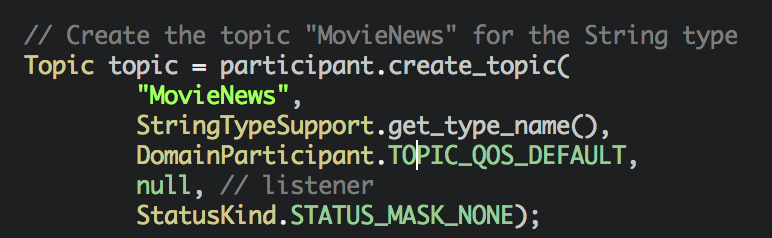
\includegraphics[width=80mm]{img/TopicCreation.png}
\caption{Creation of topic.}
\label{TopicCreation}
\end{figure}

Next up is assigning the topic to either a datawriter, or a datareader. The publisher assigns a datawriter as seen in figure \ref{CreateDataWriter}, and the subscriber assigns a datareader as seen in figure \ref{CreateDataReader}.

\begin{figure}[ht!]
\centering
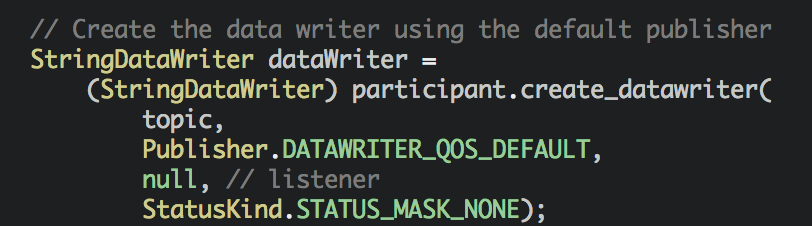
\includegraphics[width=80mm]{img/CreateDataWriter.png}
\caption{Creation of Datawriter.}
\label{CreateDataWriter}
\end{figure}

\begin{figure}[ht!]
\centering
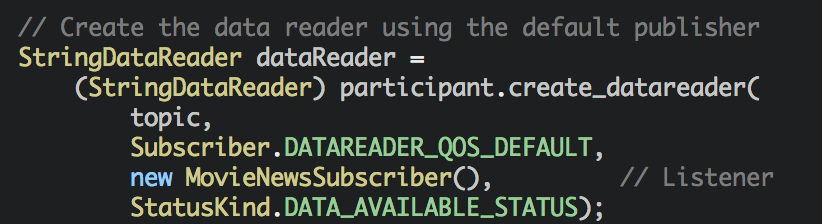
\includegraphics[width=80mm]{img/CreateDataReader.png}
\caption{Creation of Datareader.}
\label{CreateDataReader}
\end{figure}

The publisher then publishes data on the datawriter, seen in figure \ref{DataWriterWrite}. This publishes the data on the given Topic.

\begin{figure}[ht!]
\centering
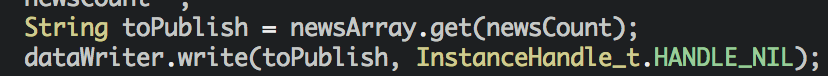
\includegraphics[width=80mm]{img/DataWriterWrite.png}
\caption{Publishing data with the Datawriter.}
\label{DataWriterWrite}
\end{figure}

The subscriber extends the class DataReaderAdapter, which enables it to implement the function on\_data\_available. This function is called when new data is published on the given topic. The specific implementation of this function is seen in figure \ref{OnDataAvailable}.

\begin{figure}[ht!]
\centering
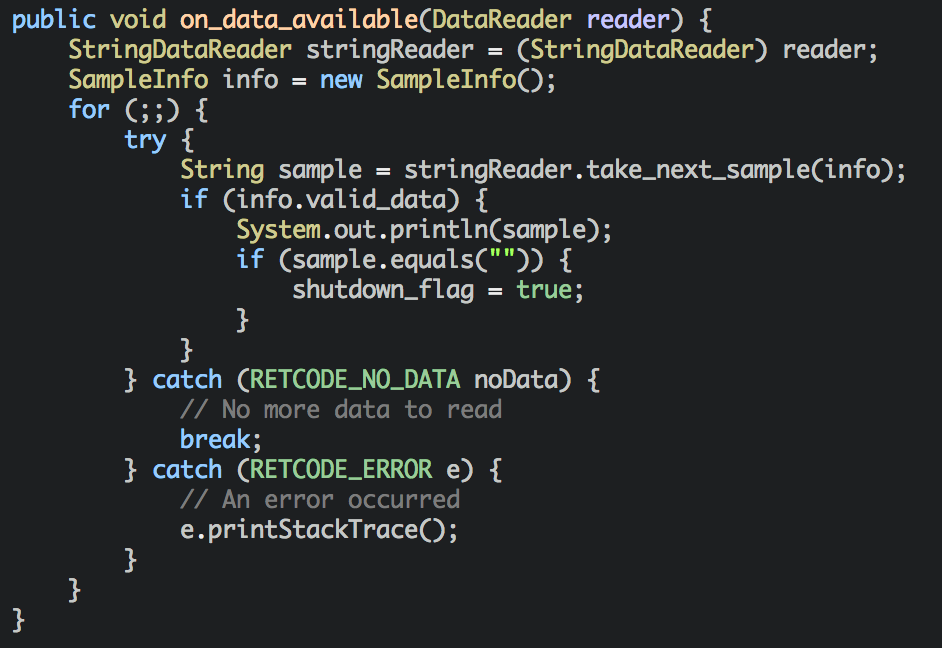
\includegraphics[width=80mm]{img/OnDataAvailable.png}
\caption{Implementation of on\_data\_available.}
\label{OnDataAvailable}
\end{figure}

Furthermore the QoS is setup in a configuration file, called \emph{USER\_QOS\_PROFILES.xml}. Examples of configuration of some of the policies are seen in the figure \ref{QOSProfiles}, in specifics it is the configuration for the datawriter. Policies as history, reliability, durability and resource limits are configured.

\begin{figure}[ht!]
\centering
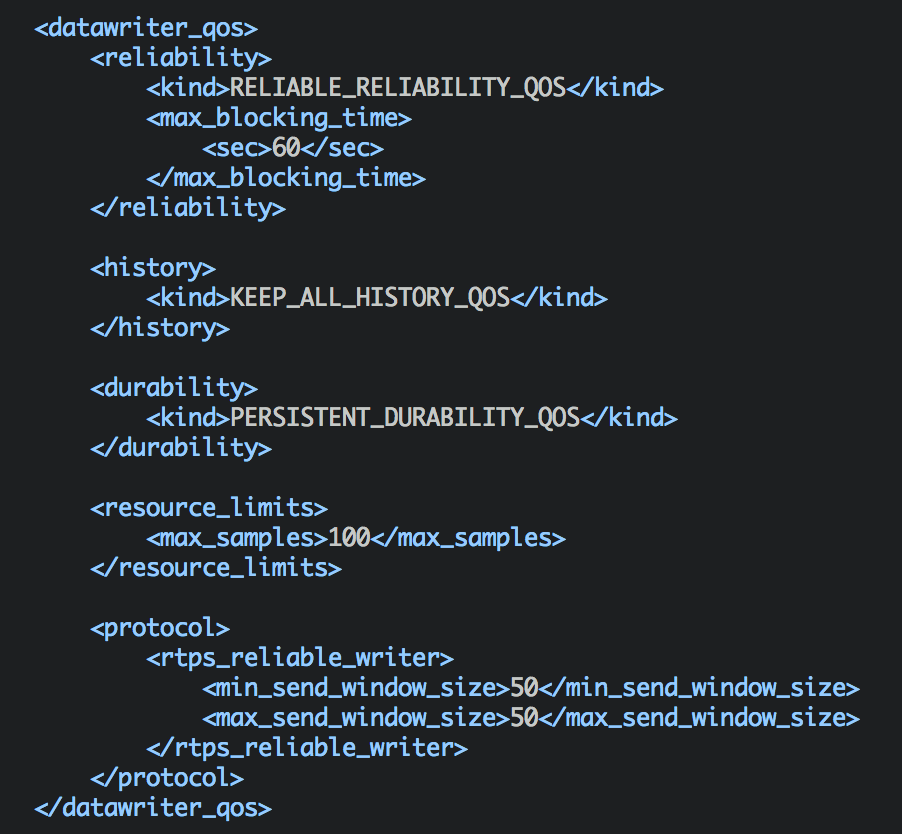
\includegraphics[width=80mm]{img/QOSProfiles.png}
\caption{QOS configuration of datawriter.}
\label{QOSProfiles}
\end{figure}

\section{Test}
To test the prototype, the four programs were run side by side. As seen in figure \ref{MovieNewsPubSub} and \ref{TechNewsPubSub}, everything works as expected. QoS history policy was also tested by opening the publisher before the subscriber, wait, and then start the subscriber.[[[[ This resulted in the subscriber getting all earlier published on the subscribed topic.]]]]

\begin{figure}[ht!]
\centering
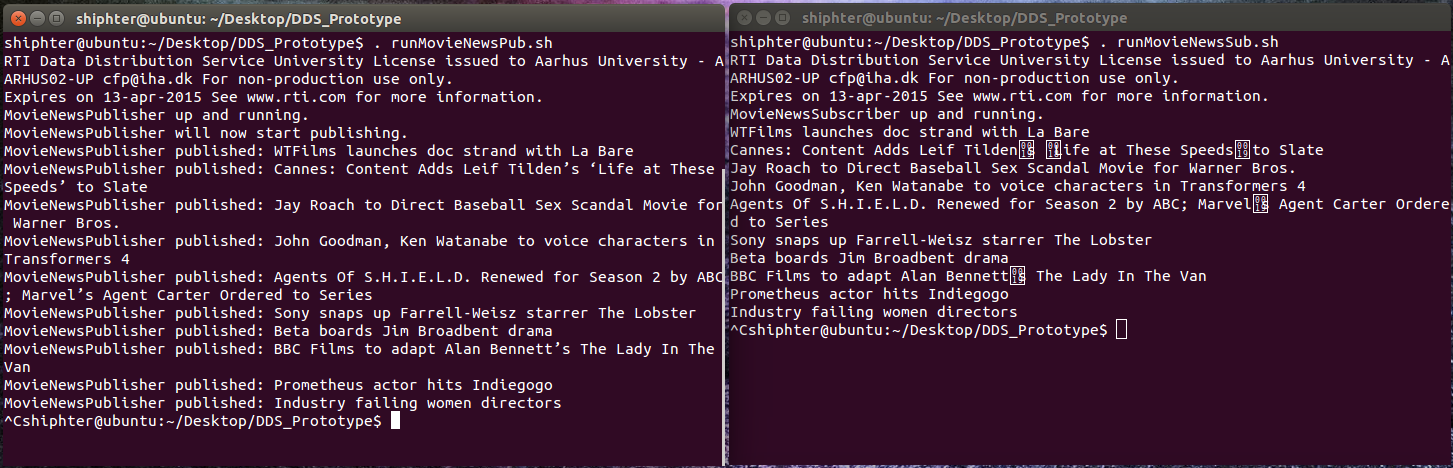
\includegraphics[width=150mm]{img/MovieNewsPubSub.png}
\caption{Test of MovieNews publisher and subscriber.}
\label{QOSProfiles}
\end{figure}

\begin{figure}[ht!]
\centering
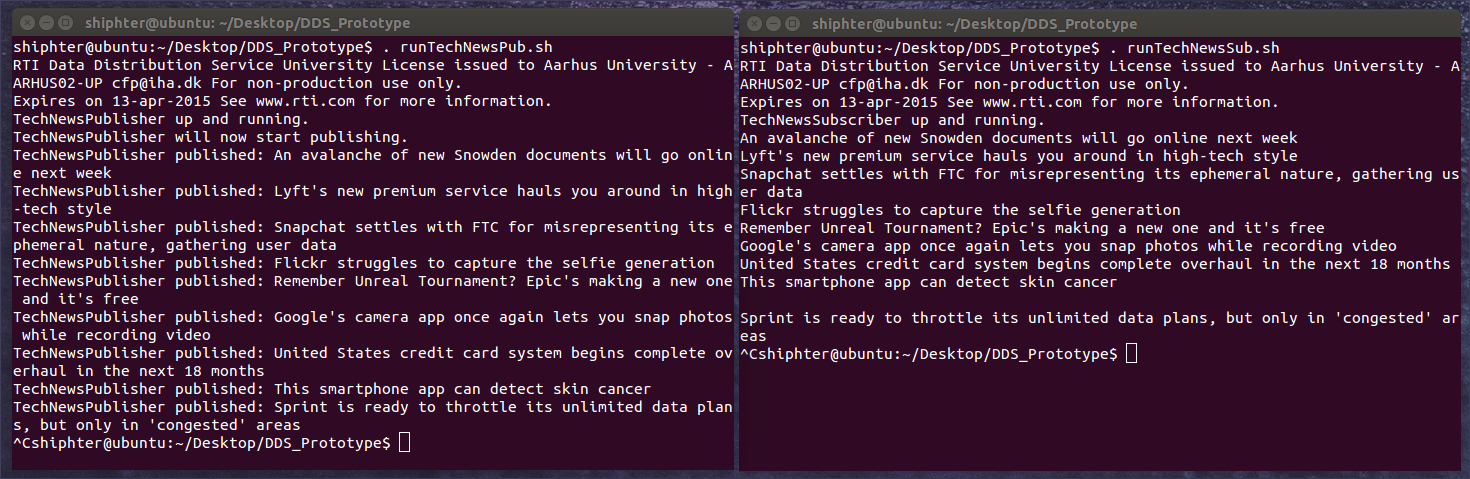
\includegraphics[width=150mm]{img/TechNewsPubSub.png}
\caption{Test of TechNews publisher and subscriber.}
\label{QOSProfiles}
\end{figure}
